\subsection{Image filtering}
possiamo prendere ad esempio chromagan (uno dei migliori modelli): l'erba la fa verde perchè è più realistica (si potrebbe pensare che ha colori anche migliori dell'originale), cartoon fa schifo perchè il modello non ha fatto un training su tali immagini, altrimenti potremmo supporre che performerebbe meglio. Infatti non riconosce l'erba come tale e sembra la colori di blu, scambiandola per acqua.
Figure \ref{fig:filter}

\begin{figure*}[t]
	\centering
	\captionsetup[subfigure]{labelformat=empty}
		\begin{subfigure}[b]{0.1\textwidth}
		\centering
		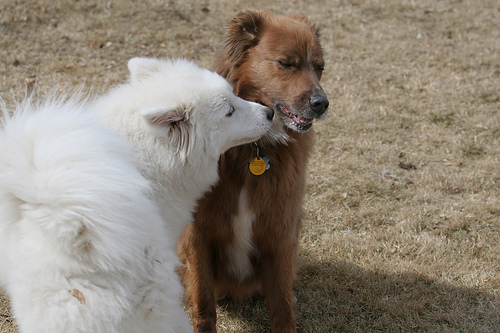
\includegraphics[width=2.4cm]{orig - filter.jpeg}
		\caption{Original}
		\end{subfigure}
		\hfill
		\begin{subfigure}[b]{0.1\textwidth}
			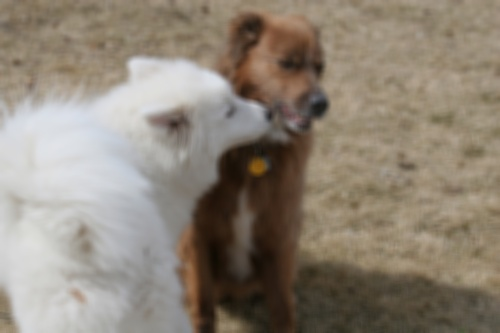
\includegraphics[width=2.4cm]{orig - filter - blur.jpeg}
			\caption{Blurred}
		\end{subfigure}
		\hfill
		\begin{subfigure}[b]{0.1\textwidth}
			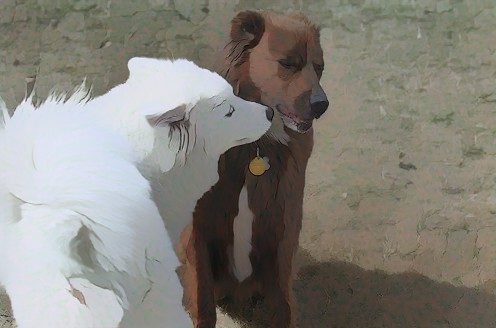
\includegraphics[width=2.4cm]{orig - filter - cartoon.jpeg}
			\caption{Cartoon}
		\end{subfigure}
		\hfill
		\begin{subfigure}[b]{0.1\textwidth}
			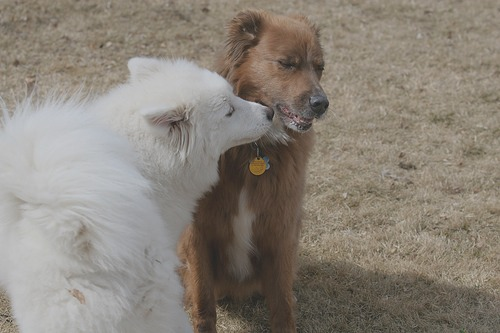
\includegraphics[width=2.4cm]{orig - filter - man contr (2).jpg}
			\caption{Low contrast}
		\end{subfigure}
		\hfill
		\begin{subfigure}[b]{0.1\textwidth}
			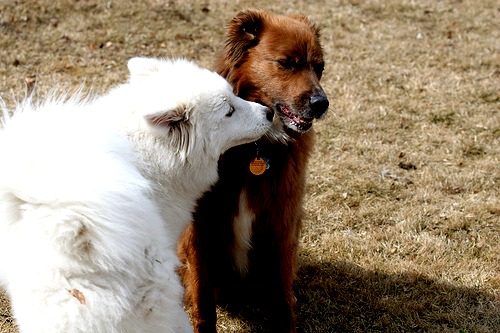
\includegraphics[width=2.4cm]{orig - filter - man contr (1).jpg}
			\caption{High contrast}
		\end{subfigure}
		\hfill
		\begin{subfigure}[b]{0.1\textwidth}
			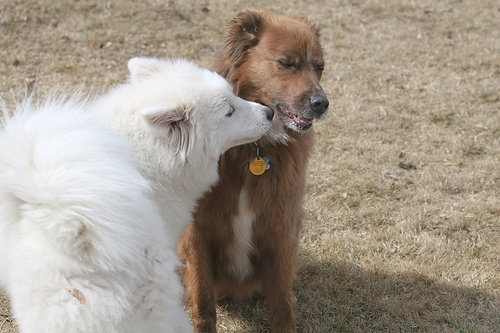
\includegraphics[width=2.4cm]{orig - filter - lumin (1).jpeg}
			\caption{Brighter}
		\end{subfigure}
		\hfill
		\begin{subfigure}[b]{0.1\textwidth}
			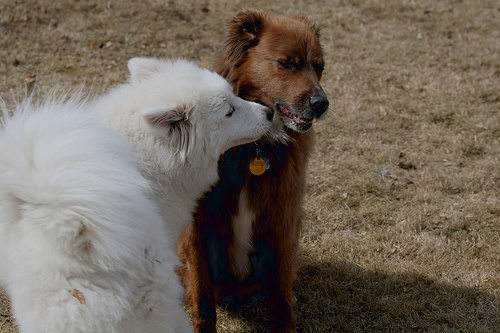
\includegraphics[width=2.4cm]{orig - filter - lumin (2).jpeg}
			\caption{Darker}
		\end{subfigure}
	
				\begin{subfigure}[b]{0.1\textwidth}
			\centering
			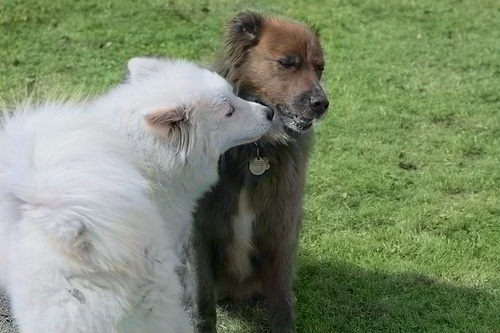
\includegraphics[width=2.4cm]{c - filter.jpeg}

		\end{subfigure}
		\hfill
		\begin{subfigure}[b]{0.1\textwidth}
			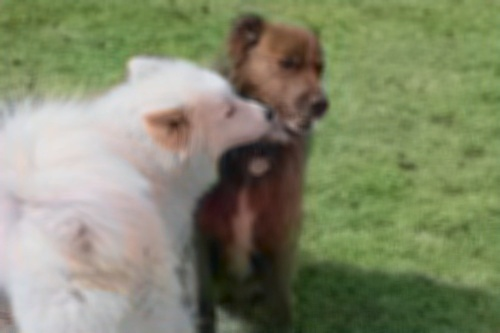
\includegraphics[width=2.4cm]{c - filter - blurr.jpeg}
		\end{subfigure}
		\hfill
		\begin{subfigure}[b]{0.1\textwidth}
			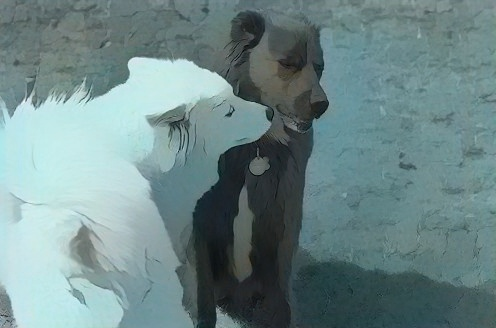
\includegraphics[width=2.4cm]{c - filter - cartoon.jpeg}
		
		\end{subfigure}
		\hfill
		\begin{subfigure}[b]{0.1\textwidth}
			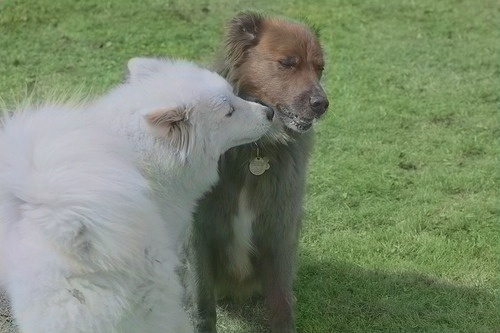
\includegraphics[width=2.4cm]{c - filter - man contr (1).jpg}
	
		\end{subfigure}
		\hfill
		\begin{subfigure}[b]{0.1\textwidth}
			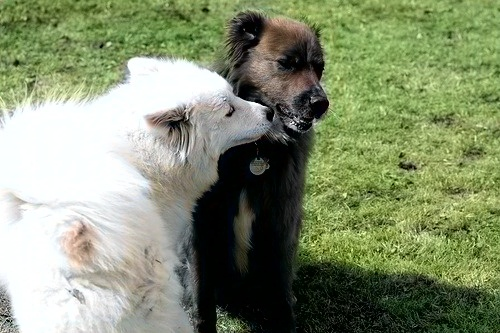
\includegraphics[width=2.4cm]{c - filter - man contr (2).jpg}
	
		\end{subfigure}
		\hfill
		\begin{subfigure}[b]{0.1\textwidth}
			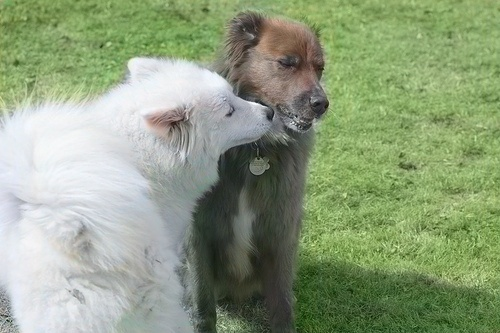
\includegraphics[width=2.4cm]{c - filter - lumin (1).jpeg}
	
		\end{subfigure}
		\hfill
		\begin{subfigure}[b]{0.1\textwidth}
			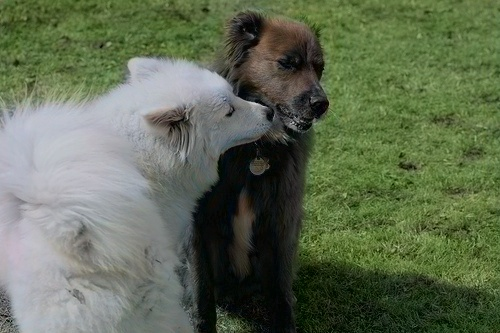
\includegraphics[width=2.4cm]{c - filter - lumin (2).jpeg}
	
		\end{subfigure}
	\caption{{\small Chromagan colorization (second row) on some filtered images (first row).}}
	\label{fig:filter}
\end{figure*}